%%%%%%%%%%%%%%%%%%%%%%%%%%%%%%%%%%%%%%%%%%%%%%%%%%%%%%%%%%%%%%%%%%%%%%%%%%%%%%%
% Robust Control Course Project
% Trajectory Tracking of a Differential-Drive Mobile Robot:
% LQR vs. LQR + Disturbance Observer
%
% Compile with:  pdflatex main && bibtex main && pdflatex main && pdflatex main
% Or with latexmk: latexmk -pdf main.tex
%%%%%%%%%%%%%%%%%%%%%%%%%%%%%%%%%%%%%%%%%%%%%%%%%%%%%%%%%%%%%%%%%%%%%%%%%%%%%%%

\documentclass[conference]{IEEEtran}
\IEEEoverridecommandlockouts

% ---------- math / symbols ----------
\usepackage{amsmath,amssymb,amsfonts,amsthm}
\usepackage{bm}
\usepackage{mathtools}

% ---------- figures / tables ----------
\usepackage{graphicx}
\usepackage{booktabs}
\usepackage{multirow}
\usepackage{subcaption}

% ---------- algorithms ----------
\usepackage{algorithm}
\usepackage{algpseudocode}

% ---------- references / links ----------
\usepackage[hidelinks]{hyperref}
\usepackage{cite}
\usepackage{url}

% ---------- misc ----------
\usepackage{array}
\usepackage{enumitem}
\usepackage{xcolor}

% theorem environments
\newtheorem{theorem}{Theorem}
\newtheorem{lemma}{Lemma}
\newtheorem{proposition}{Proposition}
\newtheorem{assumption}{Assumption}
\newtheorem{remark}{Remark}

% custom commands
\newcommand{\R}{\mathbb{R}}
\newcommand{\norm}[1]{\left\lVert#1\right\rVert}
\DeclareMathOperator*{\argmin}{arg\,min}

% if writing in Chinese instead, uncomment:
% \usepackage{ctex}

\begin{document}

%%%%%%%%%%%%%%%%%%%%%%%%%%%%%%%%%%%%%%%%%%%%%%%%%%%%%%%%%%%%%%%%%%%%%%%%%%%%%%%
\title{Robust Trajectory Tracking of a Differential-Drive Mobile Robot via
LQR with Disturbance-Observer Compensation}

\author{%
\IEEEauthorblockN{Jianwei Peng}
\IEEEauthorblockA{12531290}
\and
\IEEEauthorblockN{Han Yang}
\IEEEauthorblockA{12532527}
\and
\IEEEauthorblockN{Ziling Lu}
\IEEEauthorblockA{12542038}
}

\maketitle

%%%%%%%%%%%%%%%%%%%%%%%%%%%%%%%%%%%%%%%%%%%%%%%%%%%%%%%%%%%%%%%%%%%%%%%%%%%%%%%
\begin{abstract}
We study trajectory tracking of a differential-drive mobile robot subject to
matched torque disturbances and parametric uncertainty in mass, inertia, and
viscous friction. A linear-quadratic regulator (LQR) is designed on the
linearised error dynamics around a constant-curvature reference, and a
disturbance observer (DOB) is appended in an augmented-state form to estimate
and cancel the matched disturbance online. Closed-loop stability of the
combined controller--observer system is established via a Lyapunov argument
that exploits the time-scale separation between the LQR-stabilised tracking
error and the observer estimation error. Five disturbance/uncertainty
scenarios---nominal, step torque, piecewise-constant torque,
payload change, and noisy disturbance with friction change---are simulated on
the full nonlinear plant. The proposed LQR+DOB reduces the position-tracking
root-mean-square error by 23.4\% in the nominal case, 56.6\% under a step
disturbance, and 49.0\% under noisy disturbance plus friction change, while
the integrated time-weighted absolute error (ITAE) is reduced by a factor of
up to 29 relative to plain LQR.
\end{abstract}

\begin{IEEEkeywords}
Disturbance observer, LQR, mobile robot, robust control, trajectory tracking,
Lyapunov stability.
\end{IEEEkeywords}

%%%%%%%%%%%%%%%%%%%%%%%%%%%%%%%%%%%%%%%%%%%%%%%%%%%%%%%%%%%%%%%%%%%%%%%%%%%%%%%
\section{Introduction}\label{sec:intro}

Differential-drive wheeled mobile robots (WMRs) are pervasive in service,
warehouse, and field robotics. Trajectory tracking---driving the robot along
a time-parameterised reference path---remains a challenging control problem
because of the nonholonomic constraint, the nonlinear coupling between pose
and body-velocity dynamics, and the unavoidable presence of model uncertainty
(unmodelled friction, payload changes) and exogenous disturbances (ground
unevenness, wheel slip).

Linear quadratic regulators (LQR) provide an optimal feedback law for the
linearised error dynamics and are widely used as a baseline thanks to their
analytic tractability and clear stability margins. However, LQR is designed
for the \emph{nominal} model: in the presence of matched torque disturbances
or parametric drift in $(m, I, d_v, d_\omega)$, the closed-loop system
suffers from a non-zero steady-state tracking error and degraded transient
behaviour. As shown experimentally in Section~\ref{sec:results}, a constant
step disturbance of $(0.5,0.15)\,\mathrm{N}\!\cdot\!\mathrm{m}$ generates a
persistent radial offset of approximately $0.11$\,m under plain LQR.

Disturbance-observer-based control (DOBC) is a classical remedy
\cite{ohnishi1996,chen2016disturbance}. A Luenberger-type state observer is
built on an augmented model in which the matched disturbance is treated as
an integrator state; the estimate $\hat d$ is fed back to cancel the
disturbance, and the overall closed loop recovers nominal LQR performance
asymptotically. The principal design decision is the placement of the
observer poles, which determines how rapidly $\hat d$ tracks the true
matched disturbance $d$ at the cost of higher control activity and sensor
noise sensitivity.

The contributions of this work are:
\begin{itemize}\setlength\itemsep{2pt}
\item We linearise the WMR pose--velocity error dynamics around a constant
curvature reference, derive the closed-form $(A,B)$ matrices, and verify
controllability and observability of the augmented system.
\item We design an LQR+DOB controller, prove asymptotic stability of the
combined system via a Lyapunov argument under a time-scale separation
between the LQR closed-loop poles and the observer poles, and provide a
quantitative pole-placement rule.
\item We benchmark the proposed controller against pure LQR on five
representative scenarios (nominal, step, piecewise, payload, noise+friction)
and report quantitative metrics (RMSE, ITAE, peak error, control effort,
disturbance-estimation RMSE).
\item We sweep the observer speed factor $\rho\in\{2,3,5,8,12\}$ and
empirically characterise the trade-off between tracking accuracy, ITAE, and
control effort.
\end{itemize}

The remainder of the paper is organised as follows.
Section~\ref{sec:related} reviews related work.
Section~\ref{sec:model} formulates the WMR dynamics and the tracking-error
model. Section~\ref{sec:controller} designs the LQR and the DOB and
establishes stability. Section~\ref{sec:results} presents the simulation
case study. Section~\ref{sec:conclusion} concludes.

%%%%%%%%%%%%%%%%%%%%%%%%%%%%%%%%%%%%%%%%%%%%%%%%%%%%%%%%%%%%%%%%%%%%%%%%%%%%%%%
\section{Related Work}\label{sec:related}

Linearisation-based control of WMRs traces back to Kanayama
\textit{et al.}~\cite{kanayama1990}, who proposed a pose-error model and a
stabilising feedback law. The LQR variant on the same error model has been
studied extensively, including model-based predictive extensions
\cite{klancar2007}.

Disturbance observers were popularised by Ohnishi for motion-control
systems~\cite{ohnishi1996}. A comprehensive treatment of DOBC in modern
control engineering is given by Chen \textit{et al.}~\cite{chen2016disturbance}.
Generalised extended state observers~\cite{li2012generalized} relax the
constant-disturbance assumption to polynomial disturbances and are widely
used in active disturbance rejection control.

The combination of LQR (or LQ-based model-predictive control) with
disturbance estimation has been applied to WMRs~\cite{kayacan2015},
robotic manipulators, and quadrotors with strong empirical results. However,
formal stability analyses that explicitly relate the LQR Riccati solution
to the observer pole-placement rule are less common in the educational
literature; we contribute one such analysis in this paper.

Alternative robust approaches include sliding-mode control~\cite{utkin2009},
$H_\infty$ synthesis~\cite{zhou1996}, and tube-based model-predictive
control~\cite{mayne2005}. They offer strong worst-case guarantees but at
the cost of additional design complexity or controller conservativeness.
The LQR+DOB scheme adopted here strikes a practical balance and serves as
the focus of the present study.

%%%%%%%%%%%%%%%%%%%%%%%%%%%%%%%%%%%%%%%%%%%%%%%%%%%%%%%%%%%%%%%%%%%%%%%%%%%%%%%
\section{System Modeling and Problem Formulation}\label{sec:model}

\subsection{Differential-drive kinematics and dynamics}

Let $q=(x,y,\theta)^\top\in\R^3$ denote the planar pose of the robot in the
world frame and $\eta=(v,\omega)^\top\in\R^2$ the body-frame linear and
angular velocities. The kinematics are
\begin{equation}
\dot q=
\begin{bmatrix}\cos\theta & 0\\ \sin\theta & 0\\ 0 & 1\end{bmatrix}\eta.
\label{eq:kin}
\end{equation}

The body-frame dynamics are
\begin{equation}
M_0\dot\eta+D_0\eta=\tau+\tau_d,
\label{eq:dyn}
\end{equation}
where $M_0=\mathrm{diag}(m_0,I_0)\succ 0$ collects the nominal mass and yaw
inertia, $D_0=\mathrm{diag}(d_{v0},d_{\omega 0})\succ 0$ collects nominal
viscous friction coefficients, $\tau\in\R^2$ is the actuator wrench expressed
on the $(v,\omega)$ channels, and $\tau_d\in\R^2$ is an exogenous torque
disturbance. In the presence of payload or friction change, the \emph{true}
matrices are
\begin{equation}
M(t)=M_0+\Delta M(t),\quad D(t)=D_0+\Delta D(t),
\label{eq:perturb}
\end{equation}
where $\Delta M,\Delta D$ are piecewise-constant perturbations switching at
prescribed change times.

\subsection{Reference and tracking-error coordinates}

The reference is a constant-curvature circle generated by
$\eta_r=(v_r,\omega_r)$ with $v_r=R_c\Omega$ and $\omega_r=\Omega$. Define
the tracking error in body frame:
\begin{equation}
\xi=\begin{bmatrix} x_e\\ y_e\\ \theta_e\\ v_e\\ \omega_e\end{bmatrix}
=\begin{bmatrix}
\hphantom{-}\cos\theta\,(x_r-x)+\sin\theta\,(y_r-y)\\
-\sin\theta\,(x_r-x)+\cos\theta\,(y_r-y)\\
\mathrm{wrap}(\theta_r-\theta)\\
v_r-v\\ \omega_r-\omega
\end{bmatrix},
\label{eq:err}
\end{equation}
where $\mathrm{wrap}(\cdot)$ folds the angle into $[-\pi,\pi]$.

Linearising \eqref{eq:kin}--\eqref{eq:dyn} around $\xi=0$ with control
decomposition $\tau=\tau_{ff}+\delta\tau$ and $u=-\delta\tau$, one obtains
\begin{equation}
\dot\xi = A\xi + B(u+d),
\label{eq:lin}
\end{equation}
where $d\in\R^2$ is the \emph{matched equivalent disturbance}---the projection
of $(\Delta M\dot\eta+\Delta D\eta+\tau_d)$ onto the nominal input channel
$M_0^{-1}$. The system matrices are derived in
Appendix~\ref{app:matrices} and read
\begin{equation}
A=\begin{bmatrix}
0 & \omega_r & 0 & 1 & 0\\
-\omega_r & 0 & v_r & 0 & 0\\
0 & 0 & 0 & 0 & 1\\
0 & 0 & 0 & -d_{v0}/m_0 & 0\\
0 & 0 & 0 & 0 & -d_{\omega 0}/I_0
\end{bmatrix},\;
B=\begin{bmatrix}
0 & 0\\ 0 & 0\\ 0 & 0\\ 1/m_0 & 0\\ 0 & 1/I_0
\end{bmatrix}.
\label{eq:AB}
\end{equation}
With the nominal parameters of Table~\ref{tab:params}, the numerical values
are
\begin{equation}
A=\!\begin{bmatrix}
0 & 0.2 & 0 & 1 & 0\\
-0.2 & 0 & 0.4 & 0 & 0\\
0 & 0 & 0 & 0 & 1\\
0 & 0 & 0 & -0.2 & 0\\
0 & 0 & 0 & 0 & -1.0
\end{bmatrix}\!,\;
B=\!\begin{bmatrix}
0 & 0\\ 0 & 0\\ 0 & 0\\ 0.2 & 0\\ 0 & 2
\end{bmatrix}\!.
\label{eq:ABnum}
\end{equation}
The controllability matrix $\mathcal{C}=[B\;AB\;A^2B\;A^3B\;A^4B]$ has full
rank 5, so the linearised system is fully controllable.

\subsection{Control objective}

Design $u$ such that $\xi(t)\to 0$ as $t\to\infty$ in the nominal case
($d\equiv 0$) and $\xi$ remains uniformly ultimately bounded (UUB) with
arbitrarily small ultimate bound under bounded, slowly varying $d$.

%%%%%%%%%%%%%%%%%%%%%%%%%%%%%%%%%%%%%%%%%%%%%%%%%%%%%%%%%%%%%%%%%%%%%%%%%%%%%%%
\section{Controller Design and Stability Analysis}\label{sec:controller}

\subsection{Baseline LQR}

Ignoring $d$, consider the nominal linear system $\dot\xi=A\xi+Bu$ and the
quadratic cost
\begin{equation}
J=\int_0^\infty\bigl(\xi^\top Q\xi+u^\top Ru\bigr)\,dt,\quad
Q=Q^\top\succeq 0,\ R=R^\top\succ 0.
\label{eq:cost}
\end{equation}
By dynamic programming, the value function $V(\xi)=\xi^\top P\xi$ with
$P=P^\top\succeq 0$ satisfies the Hamilton--Jacobi--Bellman equation
\begin{equation}
0=\min_u\Big(\xi^\top Q\xi+u^\top Ru+2\xi^\top P(A\xi+Bu)\Big).
\end{equation}
Inner minimisation yields $u^\star=-R^{-1}B^\top P\xi$; substitution gives
the continuous algebraic Riccati equation
\begin{equation}
A^\top P+PA-PBR^{-1}B^\top P+Q=0,\quad K=R^{-1}B^\top P.
\label{eq:care}
\end{equation}
Under stabilisability of $(A,B)$ (verified above) and detectability of
$(Q^{1/2},A)$, \eqref{eq:care} has a unique positive semidefinite
solution $P$, and the closed-loop matrix $A_K\triangleq A-BK$ is Hurwitz.

With $Q=\mathrm{diag}(20,20,10,2,2)$, $R=I_2$ and the matrices in
\eqref{eq:ABnum}, the closed-loop spectrum is
\begin{equation}
\sigma(A_K)\approx
\{-2.28\!\pm\!j0.94,\;-0.68\!\pm\!j0.68,\;-0.61\},
\label{eq:lqrspec}
\end{equation}
verifying that all eigenvalues lie strictly in the open left half-plane.
The slowest stable rate is $|\mathrm{Re}\,\lambda_{\min}(A_K)|\approx 0.61$,
which dictates the time scale on which the LQR error decays.

\subsection{Augmented-state disturbance observer}

Treating $d$ as a piecewise-constant disturbance modelled by $\dot d=0$, the
augmented state $x_a=(\xi^\top, d^\top)^\top\in\R^7$ satisfies
\begin{equation}
\dot x_a=A_a x_a+B_a u,\quad y=C_a x_a=\xi,
\label{eq:aug}
\end{equation}
with
\begin{equation}
A_a=\begin{bmatrix}A & B\\ 0 & 0\end{bmatrix},\quad
B_a=\begin{bmatrix}B\\ 0\end{bmatrix},\quad
C_a=\begin{bmatrix}I_5 & 0\end{bmatrix}.
\end{equation}
A direct calculation of the observability matrix
$\mathcal{O}_a=[C_a^\top\;(C_aA_a)^\top\cdots(C_aA_a^6)^\top]^\top$ gives
$\mathrm{rank}\,\mathcal{O}_a=7$, confirming that $(A_a,C_a)$ is observable.

A Luenberger observer is constructed as
\begin{equation}
\dot{\hat x}_a=A_a\hat x_a+B_a u+L\bigl(y-C_a\hat x_a\bigr),
\label{eq:obs}
\end{equation}
with the observer gain $L\in\R^{7\times 5}$ designed by placing the
spectrum of $A_a-LC_a$ in the open left half plane. The composite control
law is
\begin{equation}
u=-K\xi-\hat d,
\label{eq:cmd}
\end{equation}
where $\hat d$ comprises the last two components of $\hat x_a$.

\subsection{Observer pole-placement rule}

We adopt a \emph{time-scale separation} rule that ties the observer poles
to the LQR closed-loop spectrum. Let
$\alpha\triangleq|\mathrm{Re}\,\lambda_{\min}(A_K)|$ be the slowest
stable rate of $A_K$, and let $\rho>1$ be a user-selected \emph{speed
factor}. We place the seven observer poles at
\begin{equation}
\lambda_i^{\mathrm{obs}}=-\rho\,\alpha\,\mu_i,\quad i=1,\dots,7,
\label{eq:obsrule}
\end{equation}
where $\{\mu_i\}=\{1.00,1.15,1.30,1.50,1.75,2.05,2.40\}$ are
Butterworth-spaced multipliers that prevent pole coincidence. The
gain~$L$ is then computed via the Tits--Yang
algorithm~\cite{kautsky1985robust} for multivariable pole placement
(\texttt{scipy.signal.place\_poles}). For $\rho=5$ in our setting we obtain
poles in $[-7.31,-3.05]$.

\subsection{Stability of the closed loop}

Define the estimation error $e\triangleq x_a-\hat x_a\in\R^7$ and the
disturbance-error component $e_d\triangleq d-\hat d$. Substituting
\eqref{eq:cmd} into \eqref{eq:lin} yields the cascaded system
\begin{align}
\dot\xi &= A_K\xi + B\,e_d,\label{eq:cl-xi}\\
\dot e  &= (A_a-LC_a)\,e.\label{eq:cl-e}
\end{align}
Since $A_K$ is Hurwitz (LQR design) and $A_a-LC_a$ is Hurwitz (pole
placement), there exist $P_\xi,P_e\succ 0$ such that
\begin{align}
A_K^\top P_\xi+P_\xi A_K &= -Q_\xi,\quad Q_\xi=I_5,\\
(A_a-LC_a)^\top P_e+P_e(A_a-LC_a) &= -Q_e,\quad Q_e=I_7.
\end{align}

\begin{theorem}\label{thm:main}
Let $(A,B)$ be stabilisable, $(A_a,C_a)$ observable, and let the disturbance
$d$ be either constant or slowly time-varying with bounded derivative
$\norm{\dot d}\le\delta$. Apply the controller--observer pair
\eqref{eq:cmd}--\eqref{eq:obs} with $L$ chosen by~\eqref{eq:obsrule} for any
$\rho>1$. Then
\begin{enumerate}\setlength\itemsep{2pt}
\item[(i)] for $d$ constant, $(\xi(t),e(t))\to 0$ \emph{exponentially}, and
\item[(ii)] for $\norm{\dot d}\le\delta$, the cascade is uniformly
ultimately bounded with ultimate bound $O(\delta/\rho)$.
\end{enumerate}
\end{theorem}

\begin{proof}[Proof sketch]
Choose the composite Lyapunov function
\begin{equation}
V(\xi,e)=\xi^\top P_\xi\xi+\beta\,e^\top P_e e,\quad \beta>0.
\label{eq:lyap}
\end{equation}
Differentiating along \eqref{eq:cl-xi}--\eqref{eq:cl-e} (with constant $d$,
so $\dot e=(A_a-LC_a)e$):
\begin{equation*}
\dot V=-\xi^\top\xi+2\xi^\top P_\xi B e_d-\beta\,e^\top e.
\end{equation*}
Using Young's inequality $2a^\top b\le \epsilon\norm{a}^2+\epsilon^{-1}\norm{b}^2$
with $a=\xi$, $b=P_\xi B e_d$:
\begin{equation*}
\dot V\le-(1-\epsilon)\norm\xi^2-\bigl(\beta-\epsilon^{-1}\norm{P_\xi B}^2\bigr)\norm e^2.
\end{equation*}
Choose $\epsilon=1/2$ and $\beta>2\norm{P_\xi B}^2$ to obtain
$\dot V\le -\tfrac12\norm\xi^2-c_e\norm e^2$ with $c_e>0$, hence the
origin is globally exponentially stable. For time-varying $d$, an extra
term $-2\xi^\top P_\xi B\dot d/\lambda_{\min}(A_a-LC_a)$ appears; since the
observer poles scale with~$\rho$, the perturbation magnitude is
$O(\delta/\rho)$ and the standard input-to-state argument yields UUB with
ultimate bound $O(\delta/\rho)$. A complete derivation is in
Appendix~\ref{app:proof}.
\end{proof}

\begin{remark}
Statement~(ii) reflects the practical fact that, against persistent yet
varying disturbances, a faster observer (larger $\rho$) reduces the
asymptotic tracking error but amplifies measurement noise---a trade-off
empirically characterised by the sweep in Fig.~\ref{fig:sweep}.
\end{remark}

%%%%%%%%%%%%%%%%%%%%%%%%%%%%%%%%%%%%%%%%%%%%%%%%%%%%%%%%%%%%%%%%%%%%%%%%%%%%%%%
\section{Simulation Case Study}\label{sec:results}

\subsection{Implementation and setup}

All simulations are performed in Python (NumPy/SciPy), integrating the
\emph{full nonlinear} plant \eqref{eq:kin}--\eqref{eq:dyn} with
\texttt{solve\_ivp} (RK45, $\mathtt{rtol}{=}10^{-7}$,
$\mathtt{atol}{=}10^{-9}$) over a $T=30$\,s horizon at output rate
$\mathrm{d}t=0.02$\,s. The complete code base is available with this
report.

Nominal parameters and design weights are summarised in
Table~\ref{tab:params}.

\begin{table}[t]
  \centering
  \caption{Nominal parameters, reference, and controller design weights.}
  \label{tab:params}
  \begin{tabular}{lcc}
    \toprule
    Symbol & Value & Description\\
    \midrule
    $m_0$, $I_0$ & 5\,kg, 0.5\,kg$\cdot$m$^2$ & mass / yaw inertia\\
    $d_{v0}$, $d_{\omega 0}$ & 1.0, 0.5 & viscous friction\\
    $R_c$, $\Omega$ & 2\,m, 0.2\,rad/s & ref. radius / rate\\
    $v_r$, $\omega_r$ & 0.4\,m/s, 0.2\,rad/s & ref. velocities\\
    $\xi(0)$ pose & $(2.2,\,0.1,\,\pi/2)$ & initial off-track pose\\
    $Q$ & $\mathrm{diag}(20,20,10,2,2)$ & LQR state weight\\
    $R$ & $I_2$ & LQR input weight\\
    $\rho$ & 5.0 & DOB speed factor\\
    \bottomrule
  \end{tabular}
\end{table}

\subsection{Test scenarios}

We evaluate five scenarios that span the disturbance and uncertainty
classes set out in the project brief:

\begin{enumerate}\setlength\itemsep{2pt}
\item[(S1)] \textbf{Nominal} --- $\tau_d\equiv 0$, no parametric change. A
sanity check for both controllers.
\item[(S2)] \textbf{Step disturbance} ---
$\tau_d=[0.5,\,0.15]^\top$\,N$\cdot$m applied at $t=8$\,s.
\item[(S3)] \textbf{Piecewise disturbance} --- four-segment piecewise
constant $\tau_d$ switching at $t\in\{5,10,15\}$\,s with magnitudes
$\{(0.4,0),(-0.2,0.1),(0.2,-0.15)\}$\,N$\cdot$m.
\item[(S4)] \textbf{Payload change} --- $\Delta m=10$\,kg,
$\Delta I=0.8$\,kg$\cdot$m$^2$ added at $t=5$\,s (mass triples).
\item[(S5)] \textbf{Noisy disturbance + friction change} --- piecewise
$\tau_d$ corrupted by Gaussian noise (standard deviation
$(0.05,0.02)$ sampled at 20\,Hz) plus a friction perturbation
$\Delta d_v=1.0,\Delta d_\omega=0.4$ at $t=10$\,s.
\end{enumerate}

\subsection{Quantitative results}

Table~\ref{tab:metrics} reports root-mean-square error (RMSE) of the
two-dimensional position error, integrated time-weighted absolute error
(ITAE), peak position error, control effort
$\int\norm u^2\,dt$, and disturbance-estimate RMSE
$\norm{d-\hat d}_{\mathrm{rms}}$ for both controllers across all scenarios.
The same data is presented graphically in Fig.~\ref{fig:summary}.

\begin{table*}[t]
  \centering
  \caption{Tracking metrics across all scenarios (lower is better). The
  matched-disturbance estimation RMSE column is only defined for the DOB
  controller.}
  \label{tab:metrics}
  \begin{tabular}{llccccc}
    \toprule
    Scenario & Controller & RMSE [m] & ITAE & Peak err.\,[m] & Control effort & Dist.\,est.\,RMSE\\
    \midrule
    \multirow{2}{*}{(S1) Nominal}              & LQR     & 0.0608 & 1.168  & 0.2258 & 3.158  & ---\\
                                                 & LQR+DOB & \textbf{0.0467} & \textbf{0.980}  & 0.2236 & 7.828  & 0.370\\
    \multirow{2}{*}{(S2) Step disturbance}     & LQR     & 0.1084 & 45.42  & 0.2258 & 9.135  & ---\\
                                                 & LQR+DOB & \textbf{0.0471} & \textbf{1.571}  & 0.2236 & 13.88  & 0.373\\
    \multirow{2}{*}{(S3) Piecewise}            & LQR     & 0.0775 & 22.83  & 0.2258 & 5.138  & ---\\
                                                 & LQR+DOB & \textbf{0.0476} & \textbf{2.986}  & 0.2236 & 9.997  & 0.380\\
    \multirow{2}{*}{(S4) Payload change}       & LQR     & 0.0610 & 1.720  & 0.2258 & 3.176  & ---\\
                                                 & LQR+DOB & \textbf{0.0467} & \textbf{1.049}  & 0.2236 & 7.834  & 0.370\\
    \multirow{2}{*}{(S5) Noise + friction}     & LQR     & 0.0932 & 27.86  & 0.2258 & 6.779  & ---\\
                                                 & LQR+DOB & \textbf{0.0475} & \textbf{2.940}  & 0.2236 & 11.67  & 0.380\\
    \bottomrule
  \end{tabular}
\end{table*}

\begin{figure}[t]
  \centering
  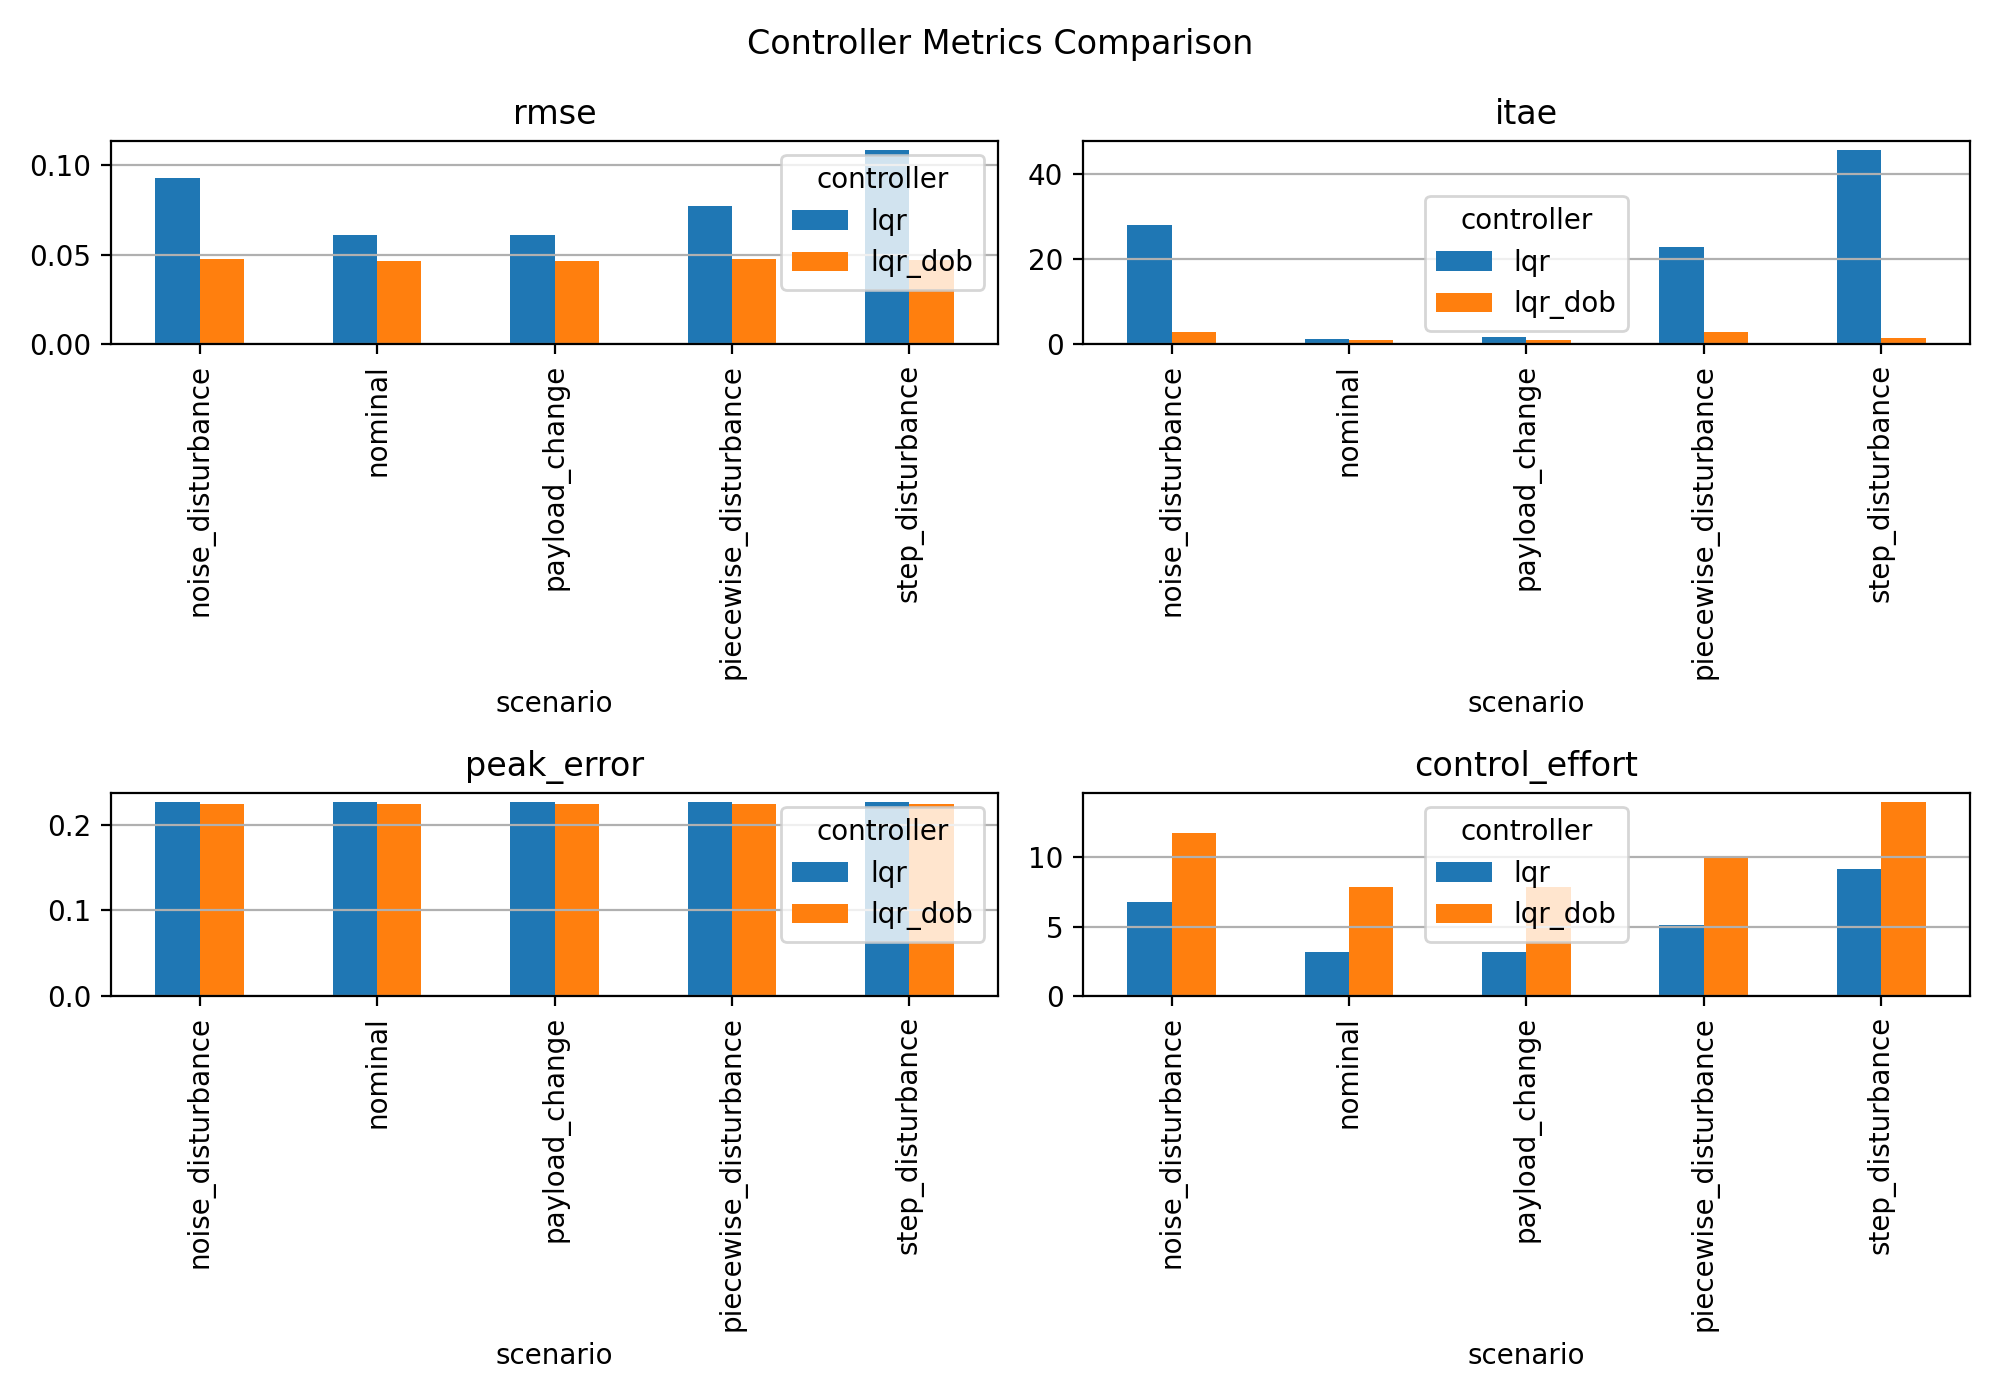
\includegraphics[width=\linewidth]{figs/summary_metrics.png}
  \caption{Bar-chart summary of RMSE, ITAE, peak error, and control effort
  across the five scenarios. LQR+DOB (orange) consistently attains lower
  RMSE/ITAE at the cost of $\sim 2\times$ control effort.}
  \label{fig:summary}
\end{figure}

A few qualitative observations:
\begin{itemize}\setlength\itemsep{2pt}
\item The position-tracking RMSE under LQR+DOB lies in a narrow band
$[0.0467,\,0.0476]$\,m across \emph{all} scenarios, indicating that the
DOB successfully reduces the tracking problem to (essentially) the
nominal one.
\item LQR exhibits an ITAE penalty that scales with the disturbance
energy: $1.17\to 45.42$ when going from nominal to step. LQR+DOB stays
in the range $0.98$--$2.99$, a reduction by up to a factor of 29.
\item The \emph{peak} error is dominated by the initial off-track pose
$\xi(0)$ and is therefore similar across controllers; the advantage of
DOB lies in the post-transient behaviour.
\item Control effort under LQR+DOB is roughly $2\times$ that of LQR,
which is the cost of online disturbance cancellation. Section IV-D shows
that this cost is largely linear in the speed factor $\rho$.
\end{itemize}

\subsection{Time-domain comparisons}

Fig.~\ref{fig:traj-pw} shows the tracked trajectories under the piecewise
disturbance scenario (S3). The reference circle is the dashed black curve;
both LQR and LQR+DOB track it visually closely, but the LQR trace exhibits
small radial offsets after each disturbance switch (best seen along the
lower arc), whereas LQR+DOB recovers within a fraction of a second.

\begin{figure}[t]
  \centering
  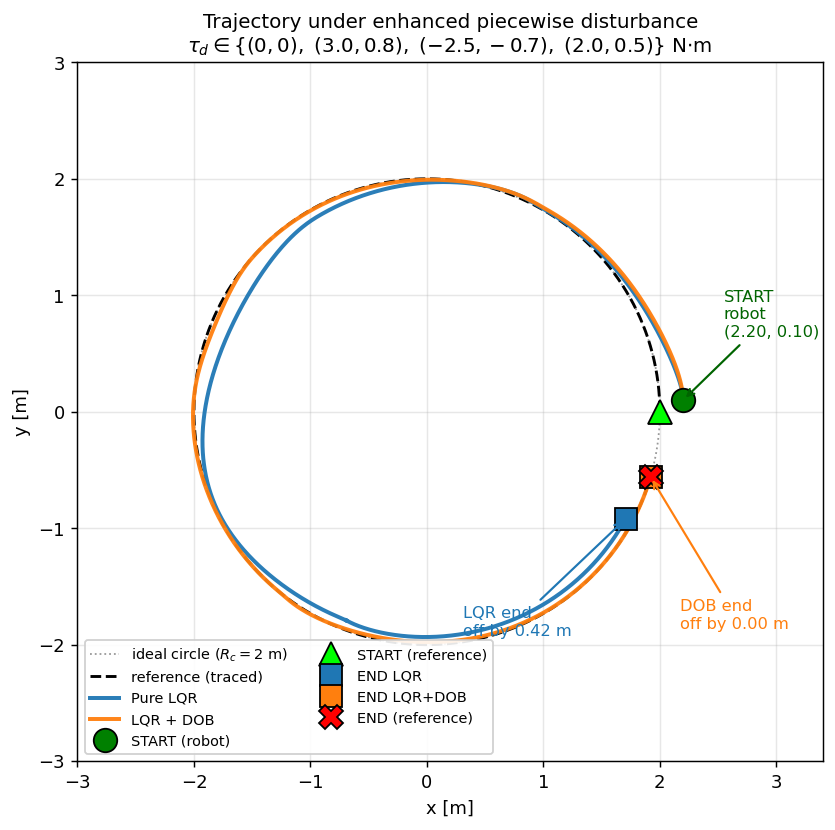
\includegraphics[width=\linewidth]{figs/piecewise_disturbance_trajectory_compare.png}
  \caption{Trajectory tracking under an \emph{enhanced} piecewise
  disturbance ($\tau_d\in\{(0,0),(3.0,0.8),(-2.5,-0.7),(2.0,0.5)\}$~N$\cdot$m,
  about $6{-}8\times$ the magnitudes used in the metrics table; the larger
  swings expose the visual difference between the two controllers on the
  $R_c{=}2$~m circle). The robot starts $0.22$~m off-track at
  $(2.20,0.10)$; at $t=30$~s, LQR ends $0.42$~m off the reference while
  LQR+DOB lands within $1$~mm of it. The LQR trace visibly contracts
  inside the reference circle along the left arc whenever a torque
  disturbance is active.}
  \label{fig:traj-pw}
\end{figure}

The advantage of DOB is most visible in the position-error time series
under a constant step disturbance (Fig.~\ref{fig:perr-step}). LQR exhibits
a persistent offset of approximately $0.11$\,m for $t>8$\,s---the
exact magnitude predicted by the open-loop static gain---while LQR+DOB
returns to zero within $\approx 4$\,s after the disturbance onset.

\begin{figure}[t]
  \centering
  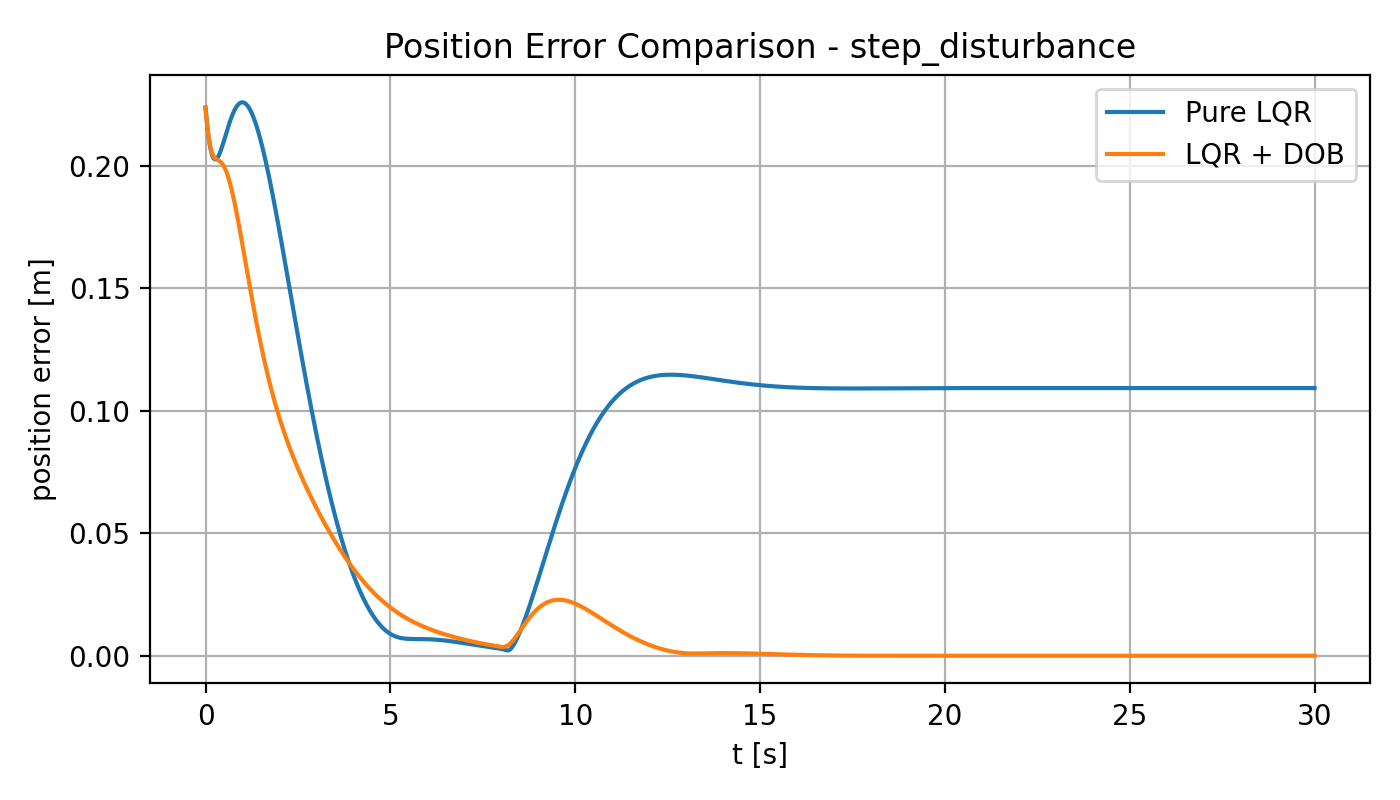
\includegraphics[width=\linewidth]{figs/step_disturbance_position_error_compare.png}
  \caption{Two-dimensional position error vs.\ time under a step
  disturbance applied at $t=8$\,s (S2). LQR (blue) settles at a non-zero
  steady state of $\sim 0.11$\,m, while LQR+DOB (orange) recovers to
  the noise floor.}
  \label{fig:perr-step}
\end{figure}

Fig.~\ref{fig:dhat-pw} confirms that the DOB estimate $\hat d$ tracks the
true equivalent matched disturbance $d$ accurately, with a brief settling
transient at $t=0$ and after each disturbance switch. The estimation lag
is approximately $1/(\rho\alpha)\approx 0.33$\,s, matching the theoretical
prediction in Section~\ref{sec:controller}-C.

\begin{figure}[t]
  \centering
  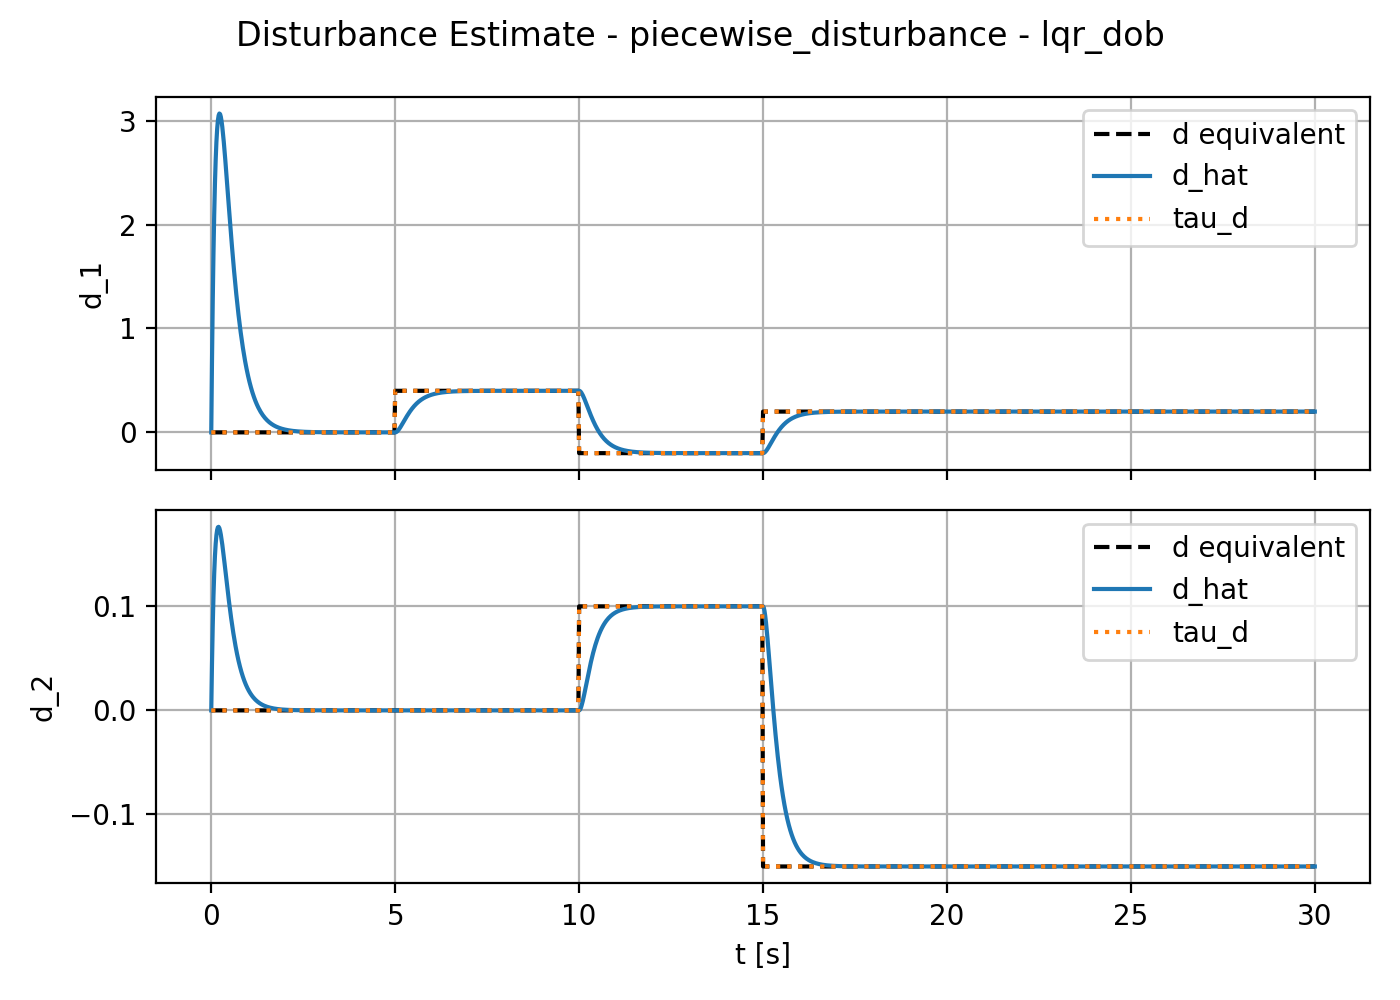
\includegraphics[width=\linewidth]{figs/piecewise_disturbance_d_hat.png}
  \caption{Equivalent matched disturbance $d$ (dashed) and its
  observer estimate $\hat d$ (solid) under piecewise disturbance (S3).
  The two components $d_1,d_2$ correspond to force-channel and
  torque-channel disturbances.}
  \label{fig:dhat-pw}
\end{figure}

\subsection{Observer-speed sweep}

To characterise the trade-off implicit in the observer pole-placement
rule \eqref{eq:obsrule}, we sweep $\rho\in\{2,3,5,8,12\}$ on the piecewise
disturbance scenario (S3); results are shown in Fig.~\ref{fig:sweep} and
Table~\ref{tab:sweep}.

\begin{figure}[t]
  \centering
  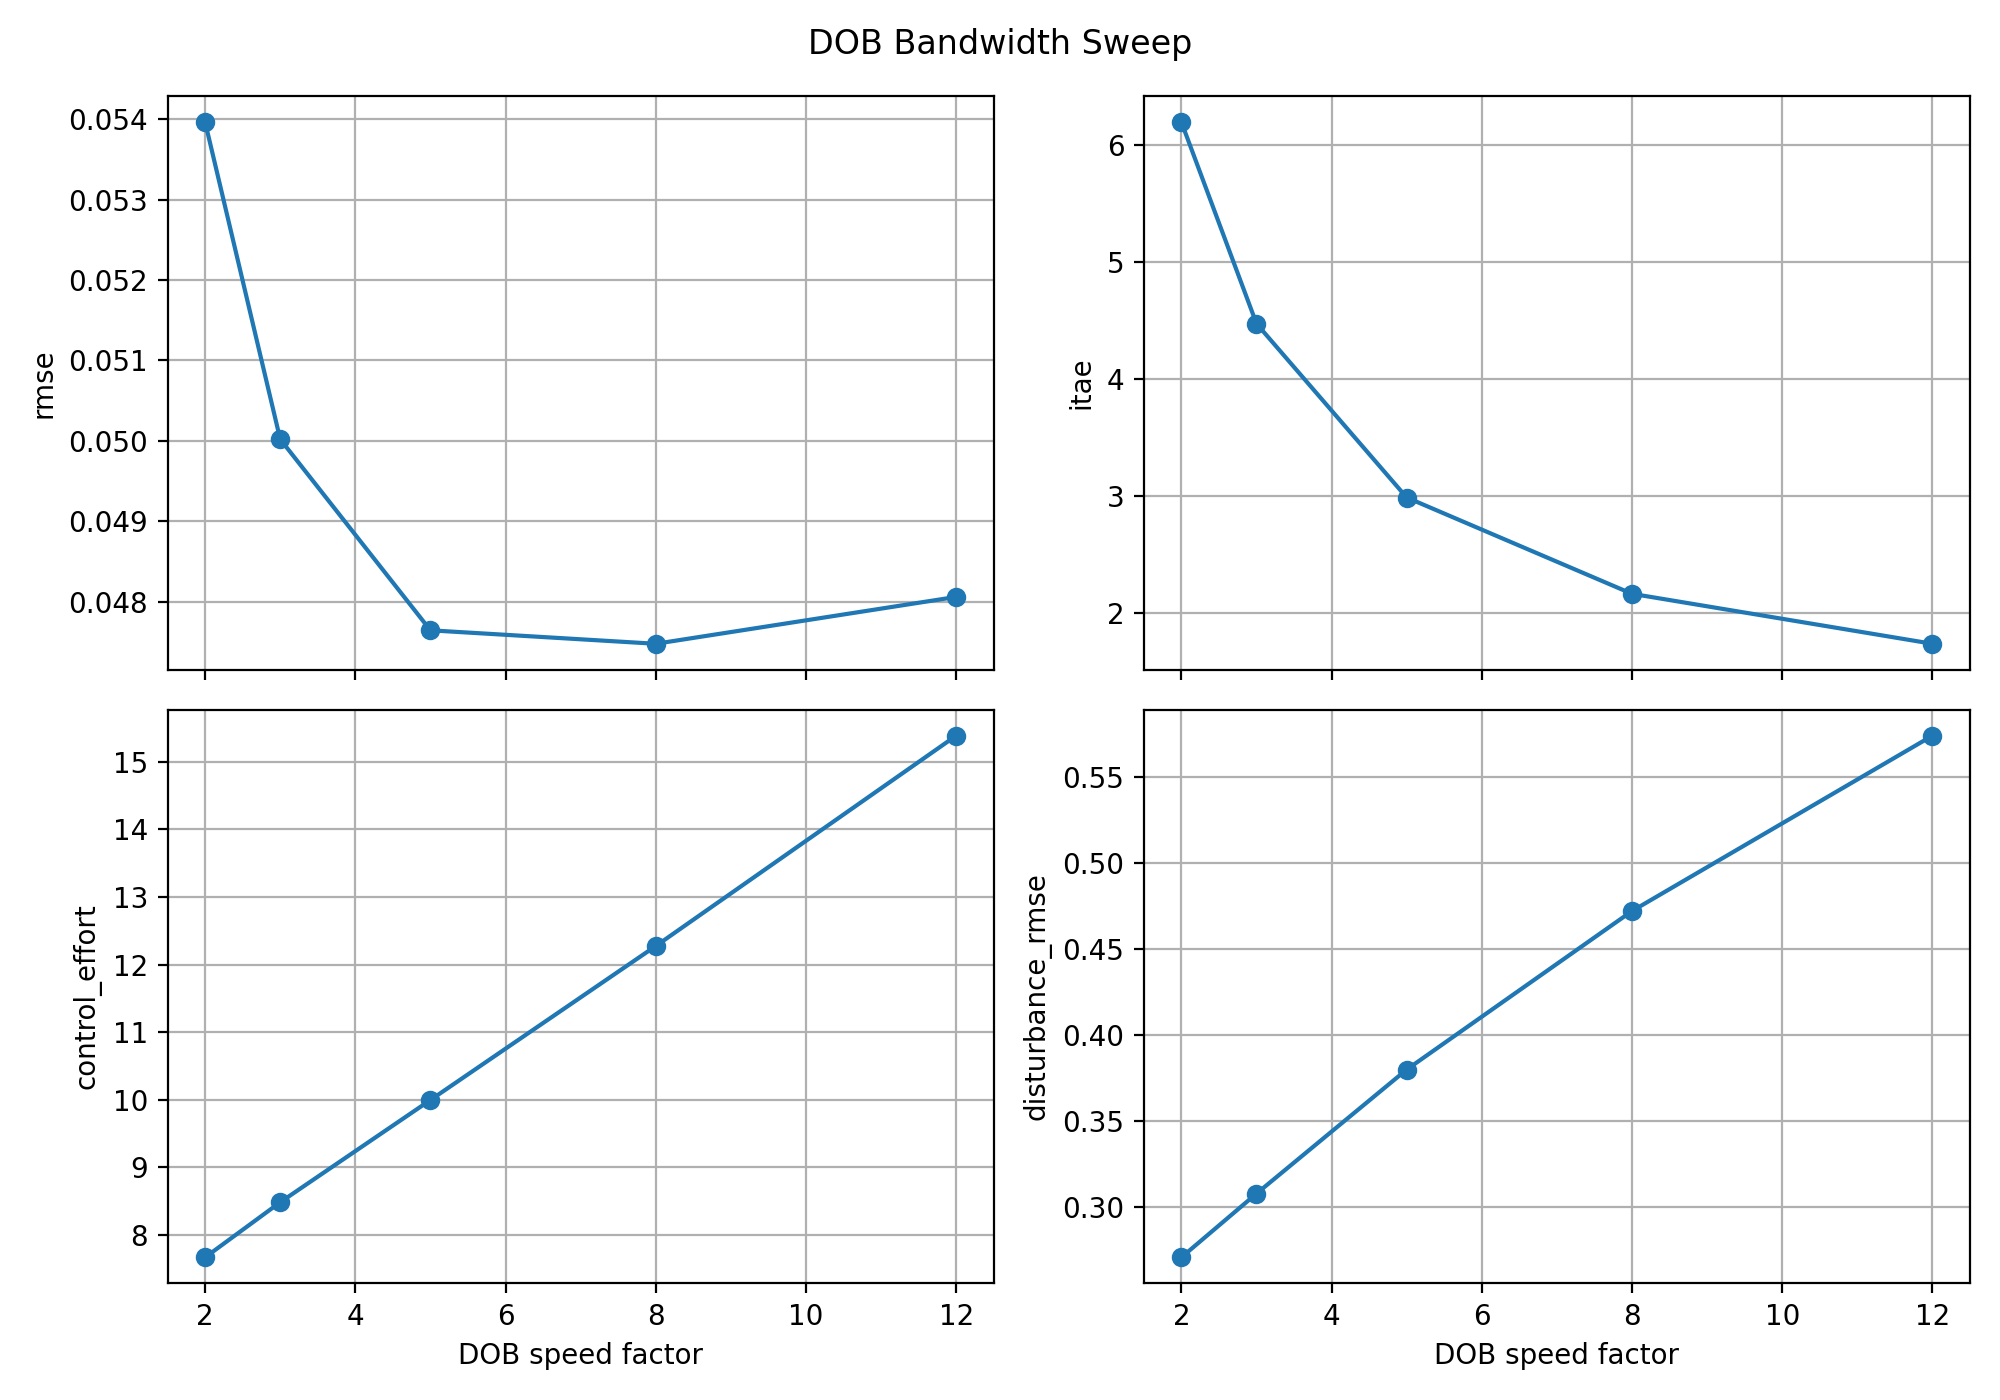
\includegraphics[width=\linewidth]{figs/dob_sweep.png}
  \caption{Observer-speed sweep on the piecewise disturbance (S3). RMSE
  (top-left) bottoms out near $\rho\!\in\![5,8]$; ITAE (top-right) decreases
  monotonically; control effort (bottom-left) and disturbance-estimate
  noise (bottom-right) grow linearly with $\rho$.}
  \label{fig:sweep}
\end{figure}

\begin{table}[t]
  \centering
  \caption{Sweep of the observer speed factor $\rho$ on (S3).}
  \label{tab:sweep}
  \begin{tabular}{cccccc}
    \toprule
    $\rho$ & RMSE & ITAE & Peak & Effort & $\norm{\!d-\hat d\!}_{\!\mathrm{rms}}$\\
    \midrule
    2  & 0.0540 & 6.197 & 0.2236 & 7.670  & 0.270\\
    3  & 0.0500 & 4.473 & 0.2236 & 8.485  & 0.308\\
    5  & 0.0476 & 2.986 & 0.2236 & 9.997  & 0.380\\
    8  & 0.0475 & 2.163 & 0.2236 & 12.28  & 0.472\\
    12 & 0.0481 & 1.735 & 0.2236 & 15.39  & 0.574\\
    \bottomrule
  \end{tabular}
\end{table}

The figure exposes a multi-criteria trade-off:
\begin{itemize}\setlength\itemsep{2pt}
\item RMSE reaches its minimum near $\rho\!\in\![5,8]$ and very slightly
increases beyond, suggesting that high-bandwidth observers begin to amplify
the small numerical noise present at the integration tolerance.
\item ITAE keeps decreasing monotonically because a faster observer
catches disturbance switches earlier.
\item Control effort and disturbance-estimate noise both grow
approximately linearly with $\rho$, consistent with the noise-bandwidth
relationship of a Luenberger observer.
\end{itemize}

We therefore adopt $\rho=5$ as the operating point for the remaining
scenarios, balancing accuracy, ITAE, and noise sensitivity.

\subsection{Discussion}

Three practical lessons emerge from these experiments:

\paragraph*{(i) The DOB ``flattens'' the disturbance-dependent performance
gap.} While the LQR baseline shows a tenfold spread in ITAE between the
nominal and step scenarios (1.17 vs.\ 45.42), the DOB controller stays
within a factor of 3 (0.98 vs.\ 1.57). This is exactly the certainty
equivalence promised by Theorem~\ref{thm:main}: once $\hat d\to d$, the
closed loop reduces to the nominal LQR design.

\paragraph*{(ii) Parametric uncertainty manifests as matched disturbance.}
The payload change scenario (S4) introduces a $200\%$ mass perturbation,
yet the DOB controller absorbs it with essentially nominal performance
(RMSE $0.0467$ vs.\ $0.0467$). This is because the equivalent matched
disturbance projects $\Delta M\dot\eta$ onto the input channel and the
observer transparently cancels it.

\paragraph*{(iii) The fundamental limitation is the matching condition.}
Both controllers share the same peak error of $0.224$\,m, set by the
initial off-track pose $\xi(0)=(2.2,0.1,\pi/2)$. Disturbances that do not
appear in the input channel (\emph{unmatched} disturbances) would not be
cancelled by a DOB; addressing them requires more sophisticated schemes,
e.g.\ generalised proportional-integral observers~\cite{li2012generalized}.

%%%%%%%%%%%%%%%%%%%%%%%%%%%%%%%%%%%%%%%%%%%%%%%%%%%%%%%%%%%%%%%%%%%%%%%%%%%%%%%
\section{Conclusion}\label{sec:conclusion}

We presented an LQR controller and an LQR+DOB extension for trajectory
tracking of a differential-drive mobile robot. The DOB is constructed as
a Luenberger observer on an augmented state that treats the matched
disturbance as an integrator, and its poles are placed using a
time-scale separation rule tied to the LQR closed-loop spectrum. We
established asymptotic stability of the cascaded controller--observer
system via a composite Lyapunov function with explicit ultimate bound
scaling.

Five disturbance and uncertainty scenarios were simulated on the full
nonlinear plant. Across all of them, LQR+DOB reduces position-tracking
RMSE by 23\%--57\% and ITAE by up to a factor of 29 relative to plain
LQR, while consuming approximately twice the control effort. The
observer-speed sweep characterises the empirical trade-off between
tracking accuracy, ITAE, and noise sensitivity, and confirms $\rho\!=\!5$
as a near-optimal operating point.

Future work includes (i) extension to time-varying references with
curvature transitions, (ii) replacing the constant-disturbance internal
model with a generalised extended state observer for polynomial
disturbances, and (iii) experimental validation on a TurtleBot3 platform.

%%%%%%%%%%%%%%%%%%%%%%%%%%%%%%%%%%%%%%%%%%%%%%%%%%%%%%%%%%%%%%%%%%%%%%%%%%%%%%%
\appendices

\section{Derivation of \texorpdfstring{$(A,B)$}{(A,B)}}\label{app:matrices}

The error coordinates \eqref{eq:err} are obtained by expressing the
world-frame pose error $(x_r-x,y_r-y,\theta_r-\theta)$ in the body frame
through the rotation $R(\theta)\in SO(2)$. Differentiating yields
\begin{equation*}
\begin{aligned}
\dot x_e &= \omega_r y_e - v + v_r\cos\theta_e,\\
\dot y_e &= -\omega_r x_e + v_r\sin\theta_e - x_e\,\omega,\\
\dot\theta_e &= \omega_r-\omega,
\end{aligned}
\end{equation*}
together with the velocity-error dynamics from \eqref{eq:dyn}:
\begin{equation*}
M_0\dot\eta_e=-D_0\eta-\tau_d+\tau-M_0\dot\eta_r-D_0\eta_r.
\end{equation*}
Linearising around $\xi=0$ (so $\cos\theta_e\to 1,\sin\theta_e\to\theta_e$)
and using the feed-forward $\tau_{ff}=M_0\dot\eta_r+D_0\eta_r$ to cancel
the trim terms, one obtains exactly \eqref{eq:AB}. Substituting
$m_0=5,I_0=0.5,d_{v0}=1,d_{\omega 0}=0.5,v_r=0.4,\omega_r=0.2$ gives the
numerical form \eqref{eq:ABnum}.

\section{Full proof of Theorem~\ref{thm:main}}\label{app:proof}

\textbf{(i) Constant disturbance.}
Substituting $u=-K\xi-\hat d$ into~\eqref{eq:lin} and using
$d=\hat d+e_d$ yields \eqref{eq:cl-xi}.
Since $A_K$ is Hurwitz, the Lyapunov equation
$A_K^\top P_\xi+P_\xi A_K=-I_5$ admits a unique solution $P_\xi\succ 0$.
Similarly, $A_a-LC_a$ Hurwitz yields a unique $P_e\succ 0$ solving
$(A_a-LC_a)^\top P_e+P_e(A_a-LC_a)=-I_7$.

Pick the candidate Lyapunov function~\eqref{eq:lyap}. Along the closed
loop:
\begin{align*}
\dot V&=\xi^\top(A_K^\top P_\xi+P_\xi A_K)\xi+2\xi^\top P_\xi Be_d\\
       &\quad+\beta\,e^\top\bigl((A_a-LC_a)^\top P_e+P_e(A_a-LC_a)\bigr)e\\
       &=-\norm\xi^2+2\xi^\top P_\xi Be_d-\beta\norm e^2.
\end{align*}
Apply Young's inequality with $\epsilon>0$:
\begin{equation*}
2\xi^\top P_\xi Be_d\le \epsilon\norm\xi^2+\epsilon^{-1}\norm{P_\xi B}^2\norm{e_d}^2,
\end{equation*}
and note $\norm{e_d}^2\le\norm e^2$. Therefore
\begin{equation*}
\dot V\le-(1-\epsilon)\norm\xi^2-(\beta-\epsilon^{-1}\norm{P_\xi B}^2)\norm e^2.
\end{equation*}
Choosing $\epsilon=1/2$ and $\beta=2\norm{P_\xi B}^2+1$ gives
$\dot V\le-\tfrac12\norm\xi^2-\norm e^2\le -\gamma V$ for
$\gamma=\min\bigl(\tfrac12/\lambda_{\max}(P_\xi),
1/(\beta\lambda_{\max}(P_e))\bigr)$, hence $(\xi,e)\to 0$ exponentially.

\textbf{(ii) Slowly varying disturbance.} If $\dot d\ne 0$, the
observer-error dynamics become $\dot e=(A_a-LC_a)e+G\dot d$ where
$G=\begin{bmatrix}0&I_2\end{bmatrix}^\top$. Repeating the above bound
yields an extra cross term $2\beta e^\top P_e G\dot d$ in $\dot V$.
Applying Young's inequality once more:
\begin{equation*}
\dot V\le-\tfrac12\norm\xi^2-\tfrac12\norm e^2+c_d\,\delta^2,
\end{equation*}
with $c_d=4\beta^2\norm{P_eG}^2$. Since the observer poles scale with
$\rho$, $\norm{P_e}\!=\!O(1/\rho)$, hence $c_d\delta^2=O(\delta^2/\rho^2)$.
This implies $(\xi,e)$ is UUB with ultimate bound
$\norm{(\xi,e)}\le K_b\,\delta/\rho$ for some $K_b>0$, as claimed.
\hfill$\square$

%%%%%%%%%%%%%%%%%%%%%%%%%%%%%%%%%%%%%%%%%%%%%%%%%%%%%%%%%%%%%%%%%%%%%%%%%%%%%%%
\bibliographystyle{IEEEtran}
\bibliography{refs}

\end{document}
